\documentclass[letterpaper,11pt]{article}
\oddsidemargin -1.0cm \textwidth 17.5cm

\usepackage[utf8]{inputenc}
\usepackage[activeacute,spanish]{babel}
\usepackage{amsfonts,setspace}
\usepackage{amsmath}
\usepackage{amssymb, amsmath, amsthm}
\usepackage{comment}
\usepackage{amssymb}
\usepackage{dsfont}
\usepackage{anysize}
\usepackage{multicol}
\usepackage{enumerate}
\usepackage{graphicx}
\usepackage[left=1.5cm,top=2cm,right=1.5cm, bottom=1.7cm]{geometry}
\setlength\headheight{1.5em} 
\usepackage{fancyhdr}
\usepackage{multicol}
\usepackage{hyperref}
\usepackage{wrapfig}
\pagestyle{fancy}
\fancyhf{}
\renewcommand{\labelenumi}{\normalsize\bfseries P\arabic{enumi}.}
\renewcommand{\labelenumii}{\normalsize\bfseries (\alph{enumii})}
\renewcommand{\labelenumiii}{\normalsize\bfseries \roman{enumiii})}

\begin{document}

\fancyhead[L]{\itshape{Facultad de Ciencias F\'isicas y Matem\'aticas}}
\fancyhead[R]{\itshape{Universidad de Chile}}

\begin{minipage}{11.5cm}
    \begin{flushleft}
        \hspace*{-0.6cm}\textbf{FI1000-5 Introducción a la Física Clásica}\\
        \hspace*{-0.6cm}\textbf{Profesora:} Paulina Lira\\
        \hspace*{-0.6cm}\textbf{Auxiliares:} Alejandro Silva, Felipe Kaschel, Juan Cristobal Castro\\
    \end{flushleft}
\end{minipage}

\begin{picture}(2,3)
    \put(405,-5){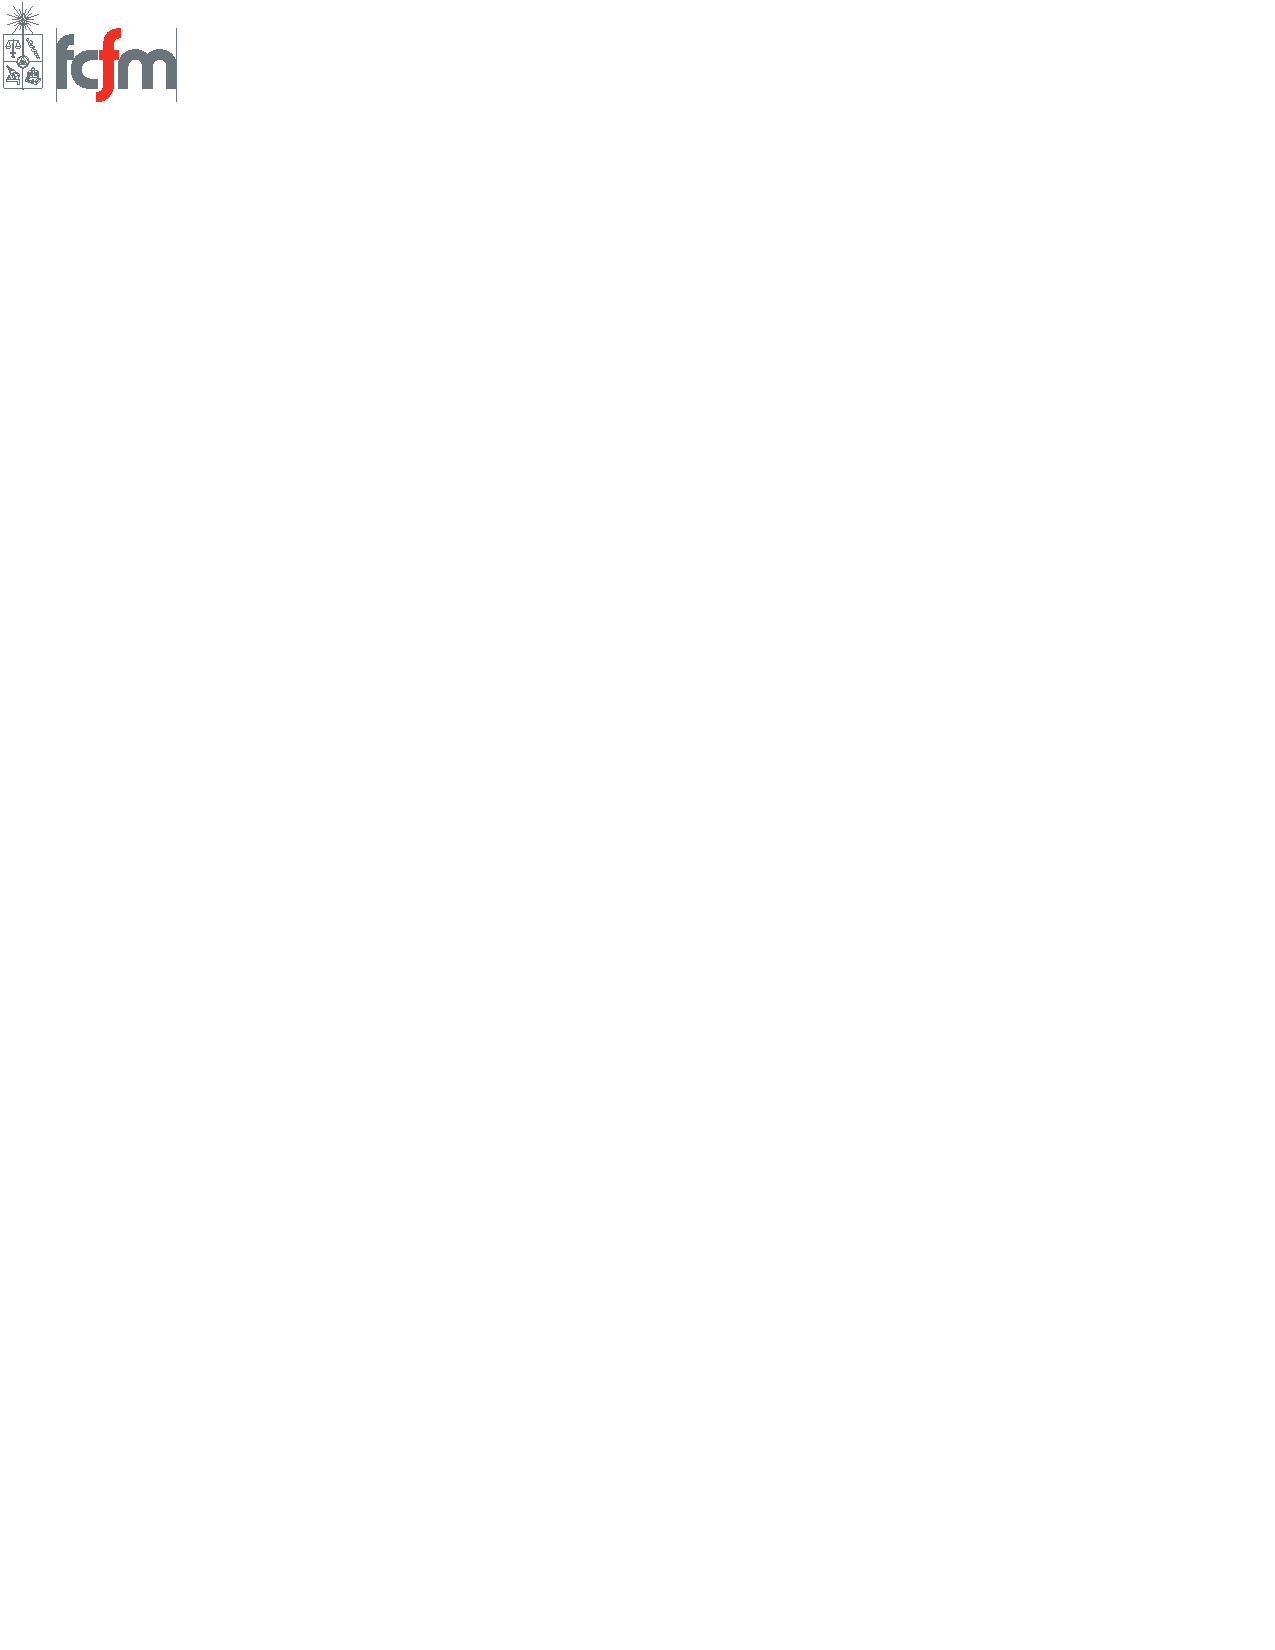
\includegraphics[scale=1.25]{2020-1/Imágenes/logo/fcfm2.pdf}}
\end{picture}

\begin{center}
	\LARGE \bf Auxiliar 4: Movimiento Circular\\
\end{center}

\vspace{-1cm}
\begin{enumerate}\setlength{\itemsep}{0.4cm}

\rfoot[]{pág. \thepage}

\item[]

\item Considere un eje vertical de largo $L$, en cuyos extremos hay dos discos sólidos provistos de ranuras. Las ranuras están desplazadas un cierto ángulo $\theta$ entre sí. El sistema gira con una velocidad angular $\omega$ constante. Calcule la altura $H$ por sobre el disco superior, desde la cual se debe soltar una bolita para que esta, en caída libre, pase por ambas ranuras.

\begin{figure}[h!]
    \centering
    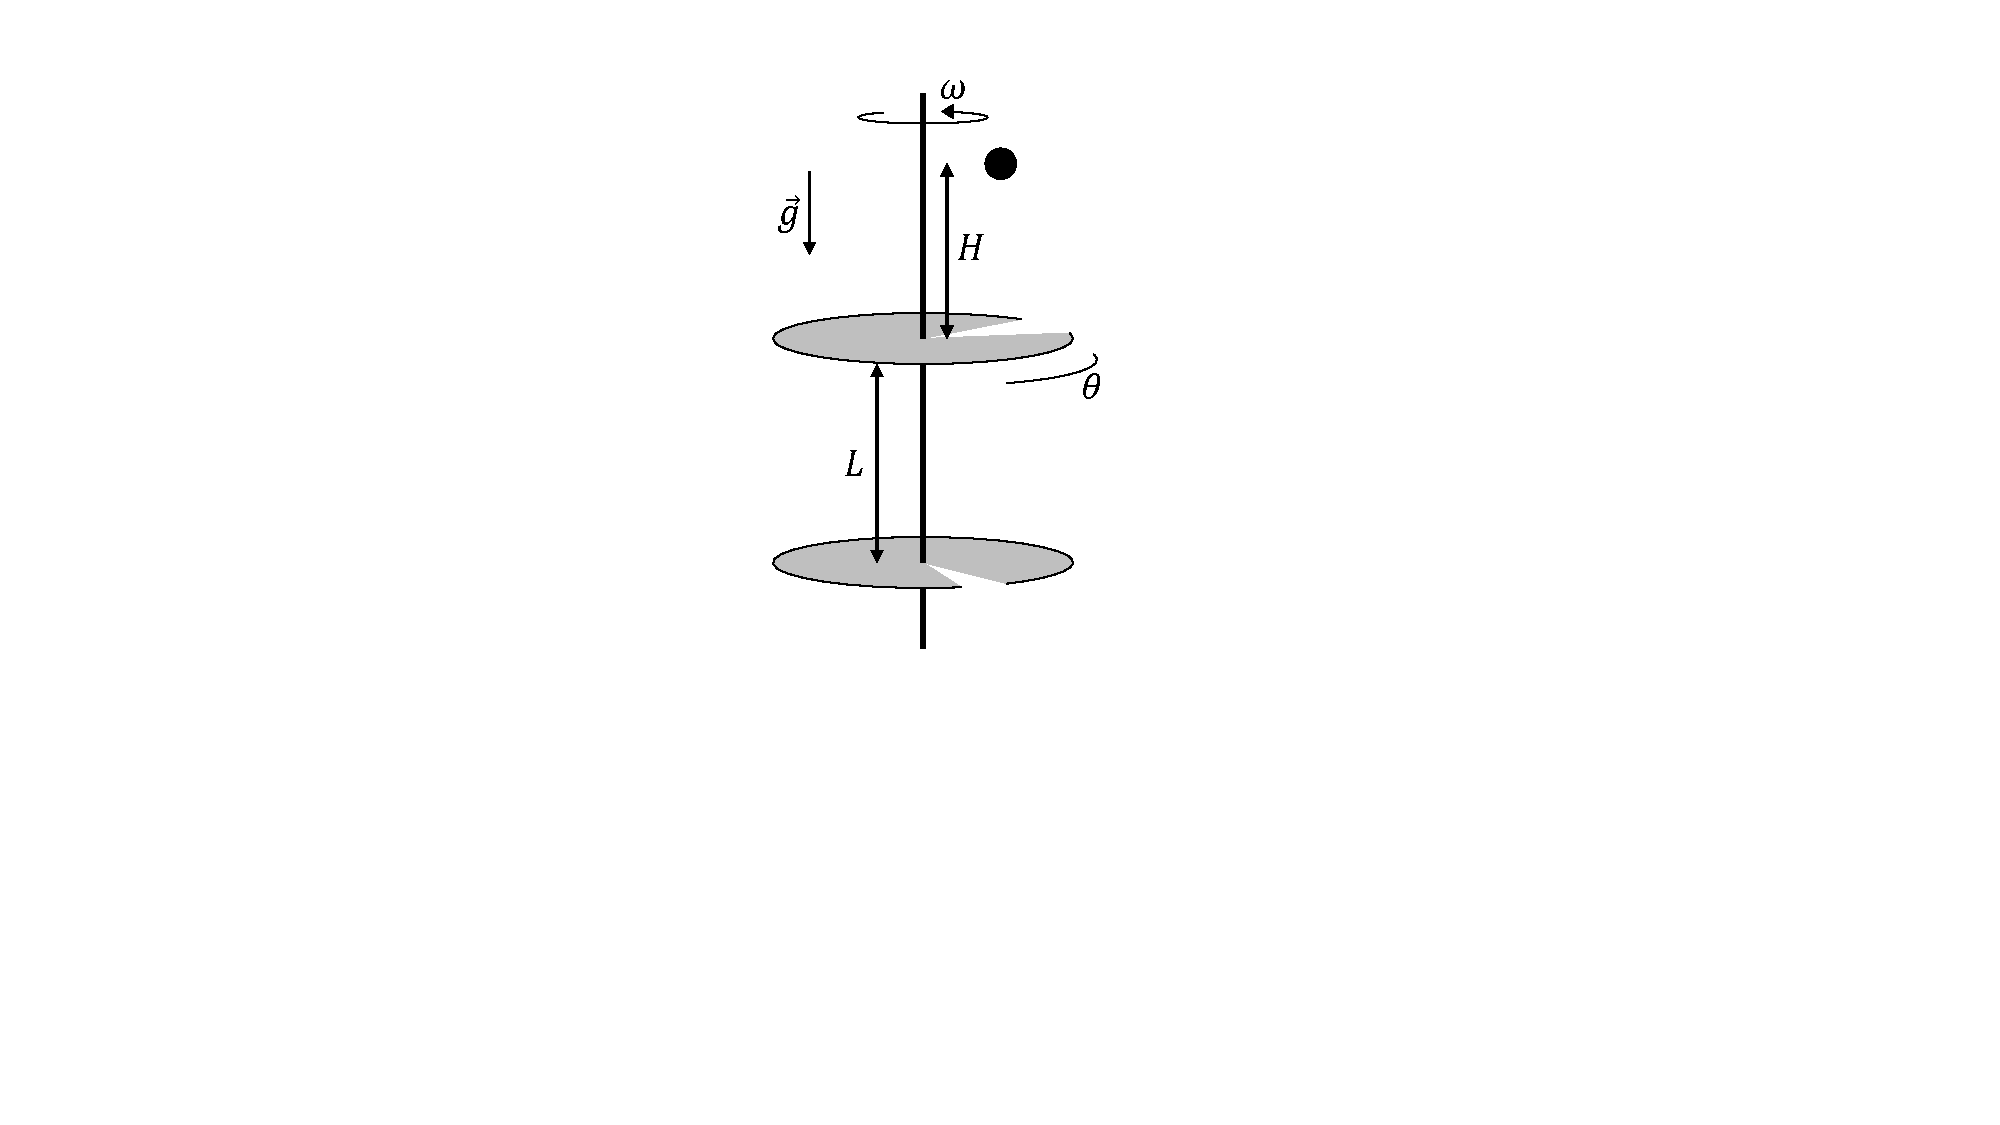
\includegraphics[scale = 0.4]{2020-1/Imágenes/aux4/vara_pelota.pdf}
\end{figure}

\item Un anillo muy pequeño se hace girar con velocidad angular constante $\omega$ a lo largo de una circunferencia vertical de radio $R$. La circunferencia está cortada en un punto determinado por un ángulo $\theta = 30^{\circ}$, como se señala en la figura. Al alcanzar este punto, el anillo se desprende y continua en caída libre.
    \begin{enumerate}
        \item Calcule el valor de la velocidad angular $\omega$ si el anillo, luego de desprenderse, toca a la circunferencia precisamente en su punto más bajo $P$
    
        \item Para el caso anterior indique la velocidad y la rapidez del anillo cuando cruza el diámetro de la circunferencia (eje $x$)
    \end{enumerate}
\begin{figure}[h!]
    \centering
    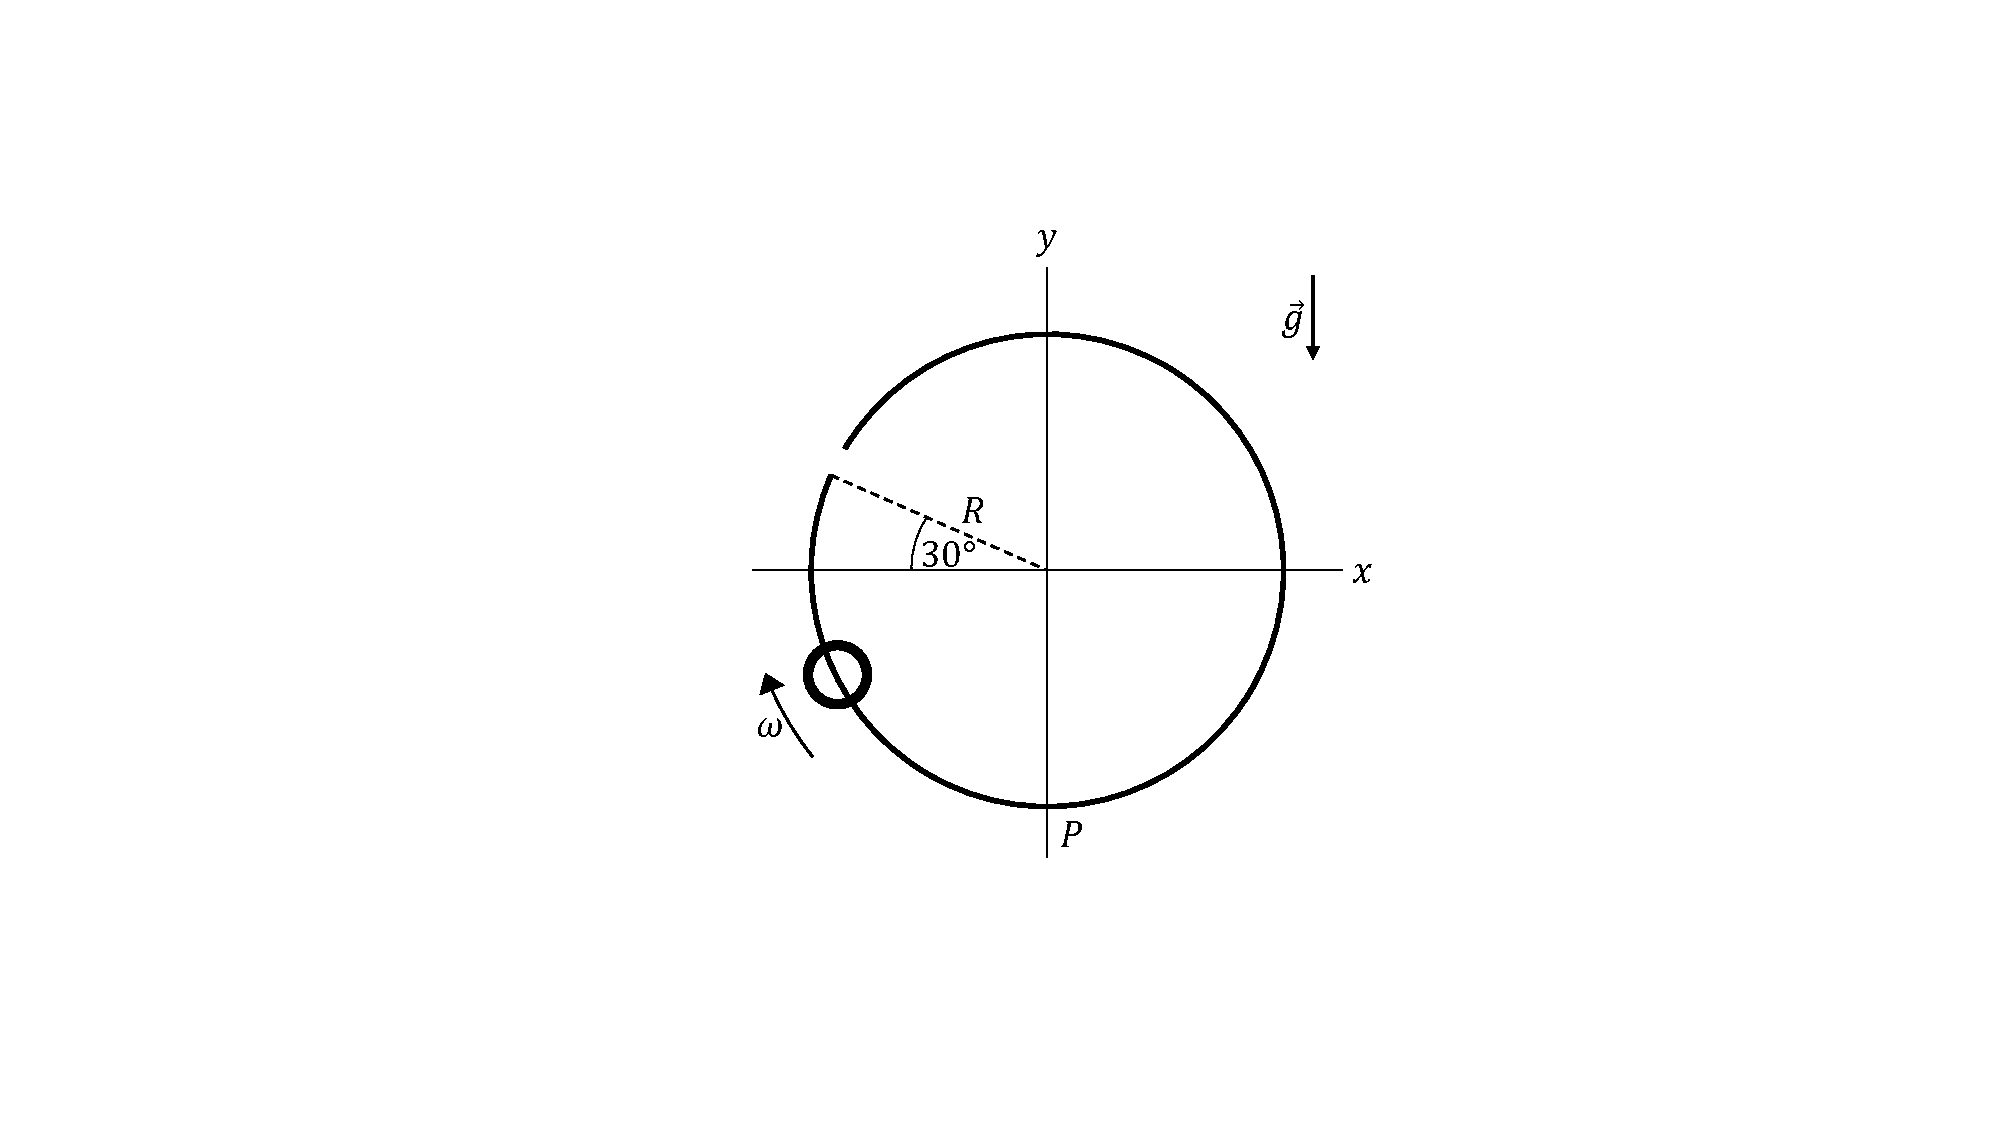
\includegraphics[scale = 0.4]{2020-1/Imágenes/aux4/circ_pelota.pdf}
\end{figure}

\item Cada lapsos de $\tau = 2.14 $ años  la distancia entre la Tierra y Marte es mínima. Suponiendo órbitas circunferenciales, uniformes y coplanares, determine el periodo de órbita de Marte en el Sistema Solar. Examine su resultado para el caso $\tau$ muy grande e interprete.

\end{enumerate}
\end{document}